\section{Sharing reproducible computational experiments}\label{sec:repro-gap}

This appendix shows how GAP code and data may be organised
in a reproducible computational experiment which can be run
on a freely available service called \href{https://mybinder.org/}{Binder}.
It demonstrates integration of a number of concepts mentioned
in the report: 
GAP regression testing (\ref{testing});
GAP Docker containers (\ref{docker});
setup for continuous integration and code coverage reports
for GAP packages (\ref{sec:package-tools}); 
and the GAP Jupyter interface (\ref{gap-4.10}).

For this demonstrator, we use the supplementary code for the 
paper \cite{black-box} by
Alexandre Borovik and \c{S}\"{u}kr\"{u} Yal\c{c}{\i}nkaya.
In this paper they present a polynomial time algorithm for 
solving a major problem in computational group theory, 
which remained open since 1999 \cite{babai-beals}. 
The code implementing is algorithm is located in the file
{\tt unipoly.g} at \url{https://github.com/sukru-yalcinkaya/unipoly}.

Presently, the authors do not intent to organise their code
in the form of a new \GAP package; nevertheless 
it can reuse packages setup for Travis CI and Codecov by 
creating a {\tt tst} directory with the test files and adapting
{\tt .travis.yml} and {\tt .codecov.yml} configuration files
from the \GAP package {\sf Example}. Connecting their repository
to Travis CI and Codecov, the authors will be able to automatically 
check that the code works in \GAP~4.9, \GAP~4.10 and 
the master branch of the GAP repository, which is a prototype for
\GAP~4.11.

\begin{figure}[!ht]
    \centering
    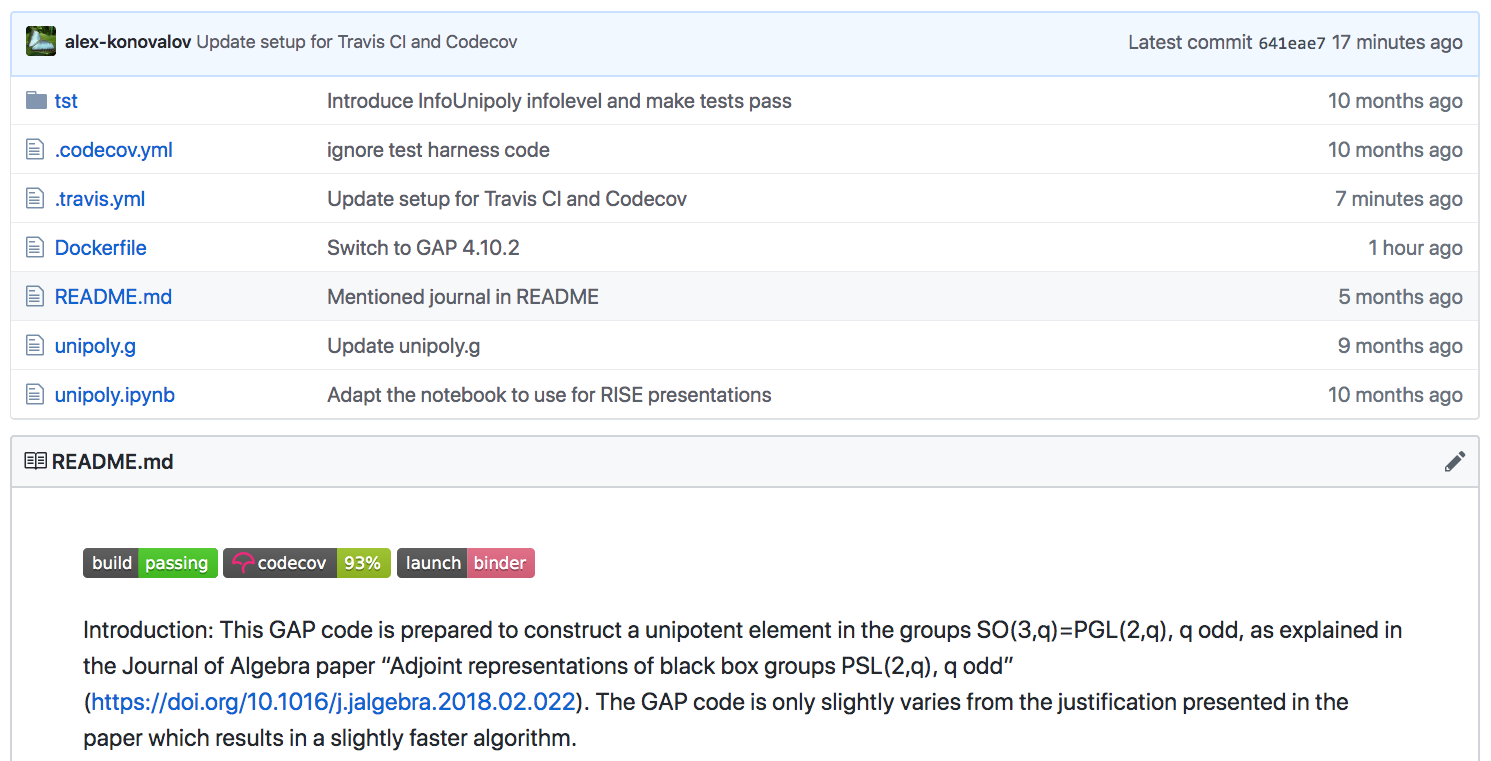
\includegraphics[width=\textwidth]{images/unipoly-repo}
    \caption{unipoly project repository}
    \label{fig:unipoly-repo}
\end{figure}

The next step is to produce a Jupyter notebook which combines input,
output, and textual narrative in one document. The notebook contains
the {\tt Read(unipoly.g);} command to read the code first. This is
a good practice for organising reproducible experiments: keeping the
code in a single location in a {\tt .g} file allows its reuse and
automated testing, and avoids code duplication. 

When the authors prepared and committed the Jupyter notebook describing
their calculation, they are ready to share it on
\href{https://mybinder.org/}{Binder}. First they need to add 
to their repository a {\tt Dockefile} with the following content:

\begin{figure}[!ht]
    \centering
    {\Small
\begin{verbatim}
FROM gapsystem/gap-docker

MAINTAINER Alexander Konovalov <alexander.konovalov@st-andrews.ac.uk>

COPY --chown=1000:1000 . $HOME/unipoly

RUN sudo pip3 install ipywidgets RISE

RUN jupyter-nbextension install rise --user --py

RUN jupyter-nbextension enable rise --user --py

USER gap

WORKDIR $HOME/unipoly
\end{verbatim}
    }
    \caption{Docker file for Binder.}
    \label{fig:pkgman-sample}
\end{figure}

This file builds a Docker container based on the container {\tt gapsystem/gap-docker}
with the latest \GAP release, which we provide as an alternative GAP distribution
(see Subsection~\ref{distro}). Additional commands specify how to copy the code into
the new container, and install additional extensions for Jupyter-based slideshows.

After that one should follow \href{https://mybinder.org/}{Binder} instructions to
set up a new Binder project. A completed setup will allow to click on the ``launch binder''
button in the README file on GitHub (as seen on Figure~\ref{fig:unipoly-repo}
to start a Jupyter notebook server in the cloud,
either using a prebuilt image of the project or by building a new one in case of any
changes in the GitHub repository. When the server will be started, it will display
a file browser as shown on Figure~\ref{fig:unipoly-files}.

\begin{figure}[!ht]
    \centering
    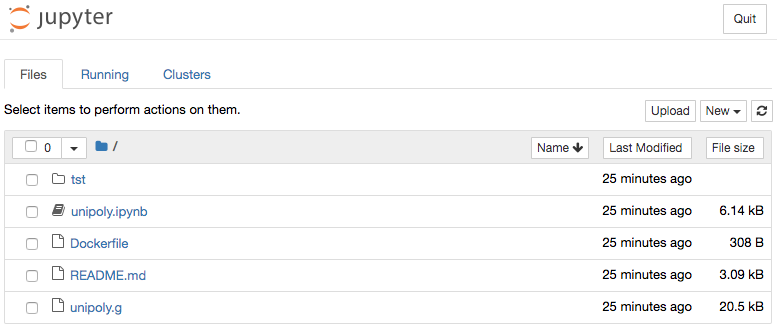
\includegraphics[width=\textwidth]{images/unipoly-files}
    \caption{File browser running on Binder}
    \label{fig:unipoly-files}
\end{figure}

Clicking on {\tt unipoly.ipynb}, the user will open the Jupyter notebook
and will be able to rerun it as shown on Figure~\ref{fig:unipoly-notebook}.

\begin{figure}[!ht]
    \centering
    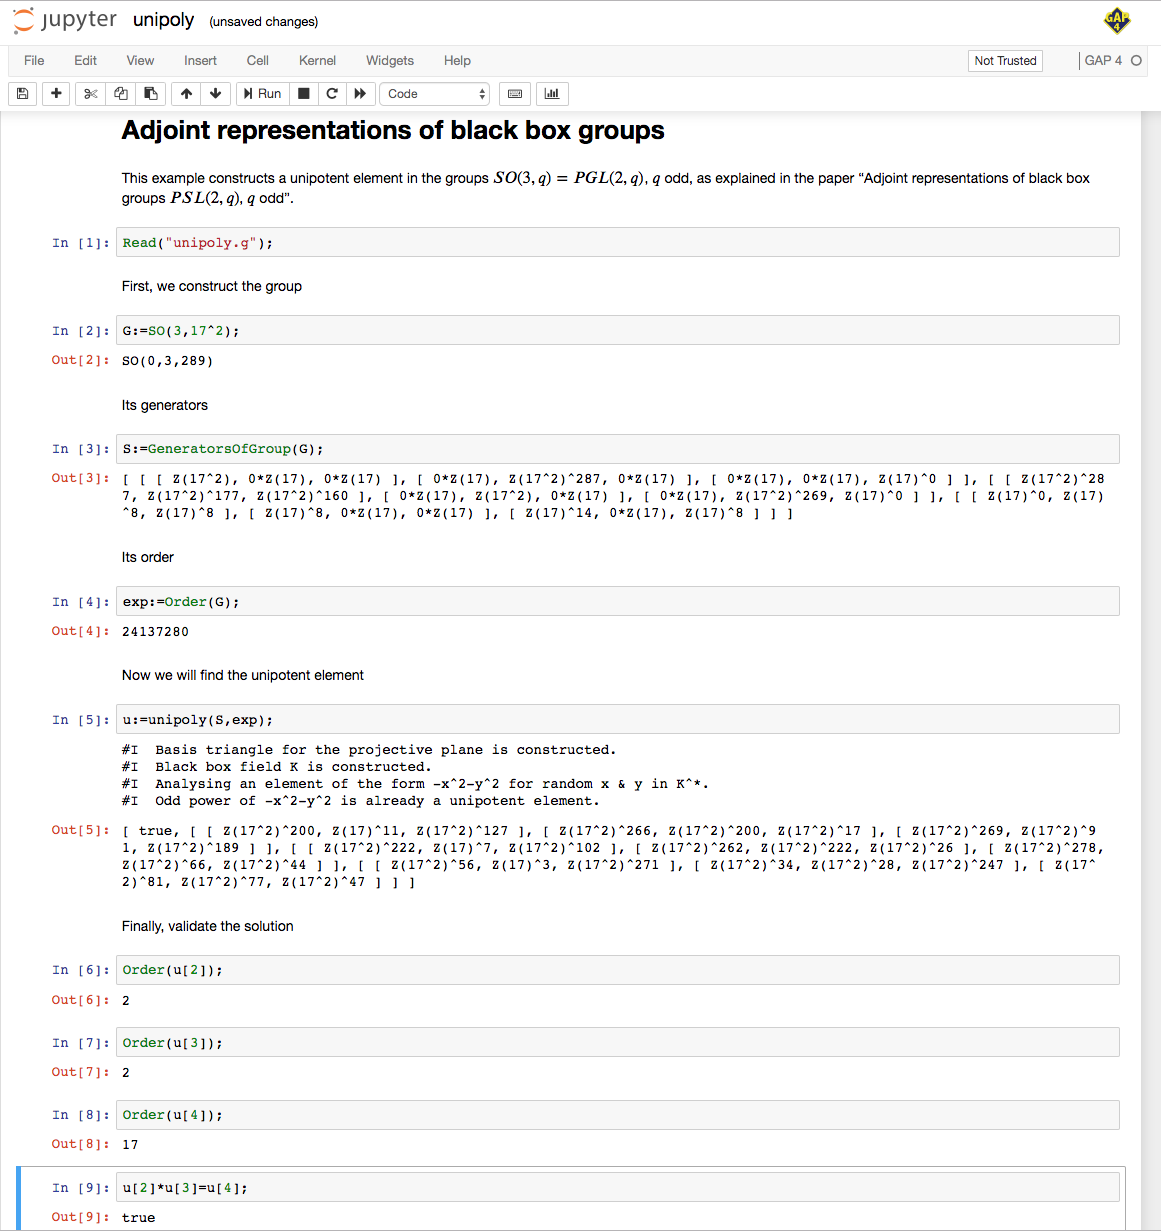
\includegraphics[width=\textwidth]{images/unipoly-notebook}
    \caption{Jupyter notebook running on Binder}
    \label{fig:unipoly-notebook}
\end{figure}

One could also switch to the slideshow mode (the notebook would require
some configuration to explain which cells should be displayed on the
same slide and which not), and run an interactive presentation, as
as shown on Figure~\ref{fig:unipoly-slide}.

\begin{figure}[!ht]
    \centering
    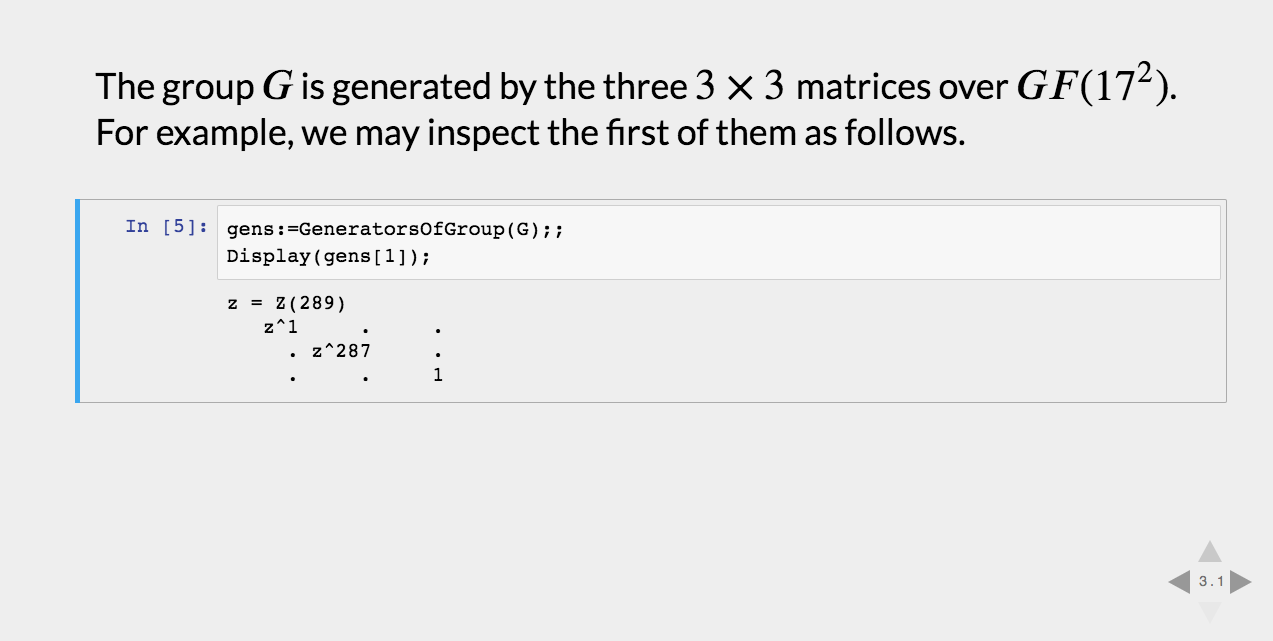
\includegraphics[width=\textwidth]{images/unipoly-slide}
    \caption{Slideshow with interactive computation running on Binder}
    \label{fig:unipoly-slide}
\end{figure}

Thus, connecting the project repository to Binder allows other users
(e.g. readers or referees of the paper) to rerun computations on Binder
without spending efforts on installing all necessary components
(may be hard for them as non experts, may not always be possible;
something may not work on Windows, etc.

\TODO{what are the limitations of Binder and suggested workarounds}
